\section{Introducción}

Las redes de monitoreo de calidad del aire de alta densidad son una necesidad creciente de las áreas urbanizadas. Estas permiten monitorear la calidad del aire a escala local, generando información vital para la toma de desiciones en áreas de salud pública. Al incrementar la cantidad de estaciones de monitoreo, la resolución de los datos aumenta, pero también aumentan el costo, la infraestructura y el personal necesario para atenderlas\cite{urban_air_quality}. De la misma forma, la demanda para redes de monitoreo climatológico de alta densidad ha ido en aumento por su utilidad en la medición de los impactos de las políticas de control en el ambiente\cite{muller_sensors_and_the_city}.

Las instalaciones de monitoreo meteorológico eran acostumbradas a ubicarse en las afueras de complejos ubranizados, centrados en la recolección de información para un análisis a escala global de los datos climatológicos, tales como el análisis del calentamiento global y los índices de radiación, así como otros datos importantes. Debido a los cambios en las necesidades de calidad y cantidad de datos, esto ha cambiado significativamente\cite{oke_2004}.

Las estaciones de monitoreo climatológico funcionan de la misma forma que la mayoría de los servidores en el mercado; Un equipo de cómputo que está corriendo un servicio escucha constantemente las peticiones de los clientes a los que está conectado, creando y actualizando datos conforme es necesario. El equipo de cómputo además se conecta a sensores que utiliza para el monitoreo contínuo de datos, los procesa, y los almacena para su posterior análisis. Esto, crea la posibilidad de integrar y crear sistemas de monitoreo de equipos de cómputo para el monitoreo de la salud de las estaciones

\pagebreak

\section{Planteamiento del problema}

\subsection{Antecedentes}

El desplegar y mantener una red meteorológica urbana compone bastantes retos: Entre la creciente dificultad de crear **sistemas** de medición estandarizados que se adapten al siempre cambiante paisaje urbano; como la instalación de los equipos de medición y de guardado de datos en áreas que permitan acceso para mantenimiento y que sean seguros; y la dificultad de encontrar un punto de acceso a internet adecuado para transferir la información generada, el generar una red de monitoreo es una tarea extensa y compleja.

Debido a estos retos, la comunidad de monitoreo climatológico y meteorológico se ha enfocado en la creación de sistemas que sean más eficientes y económicos. Entre estos esfuerzos, se encuentra el amplio uso de RaspberryPi como centro de recolección de datos de estaciones de monitoreo\cite{rpi_weataher_station}, tanto caseras como profesionales, con la ayuda de sistemas abiertos para la recolección de datos como lo es WeeWX. Esto ha hecho factible el **levantar** redes de 50 nodos de monitoreo de sensores económicamente viables para actores con un presupuesto limitado\cite{monitoreo_raspberry_nagios}.

% TODO Agregar sección de monitoreo de Campbell, y como funciona actualmente

Estas redes densas requieren de un monitoreo contínuo para mantener una alta calidad de los datos recabados, y evitar las pérdidas por falta de mantenimiento. Entre los sistemas de monitoreo que pueden ser adaptados para el monitoreo de estaciones meteorológicas y la red que las soporta, se encuentra la plataforma Nagios®, el cual es un sistema de monitoreo contínuo orientado a redes y servidores. Entre la información que recaba Nagios contínuamente para el estado de los servidores, se encuentra el uso de CPU y RAM, así como estado de los discos, puertos, e información variada de servicios de red en los hosts. Debido a que Nagios es un sistema de monitoreo de redes orientado a profesionales de la informática, la interfaz gráfica es poco amigable con los usuarios menos familiarizados con los conceptos técnicos de los sistemas computacionales\ref{fig:nagios_dashboard}.

\begin{figure}[!ht]
	\centering
	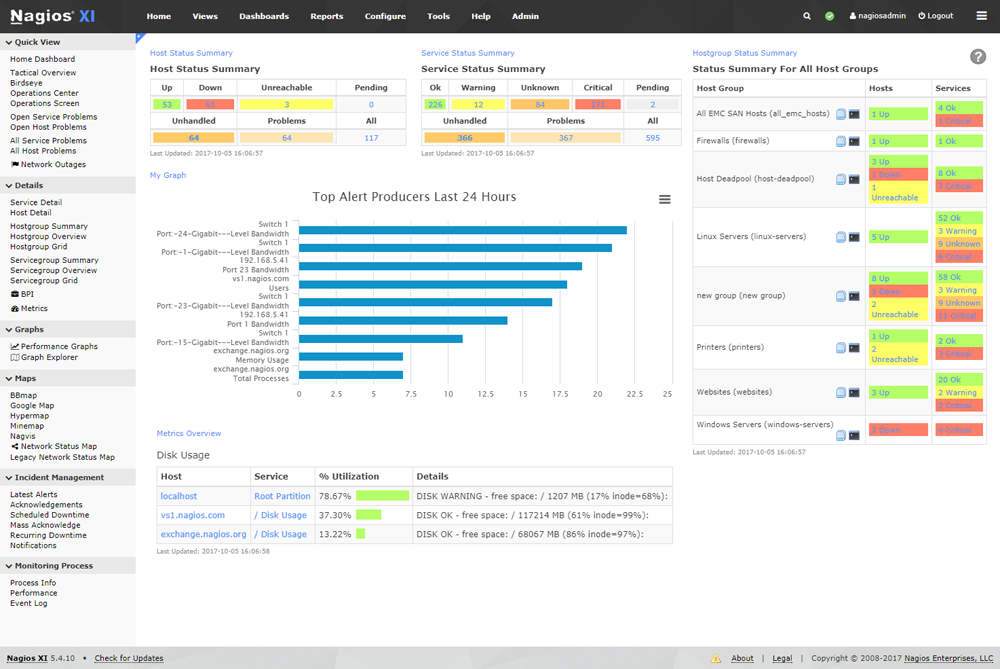
\includegraphics[width=.80\linewidth]{images/Nagios_home_dashboard.png}
	\caption{Tablero principal de Nagios XI.}
	\label{fig:nagios_dashboard}
\end{figure}

Si bien Nagios ofrece la posibilidad de monitorear parámetros adicionales con un sistema establecido de plugins en python y otros lenguajes, además de poseer una fuerte comunidad que crea contínuamente plugins relacionados con el proyecto, hasta el momento la cantidad de plugins relacionados con estaciones meteorológicas existentes es mínima ya que los esfuerzos de la comunidad se centran principalmente en el monitoreo de centros de datos y routers.

Además de los plugins existentes en la comunidad de Nagios, existe la alternativa abierta conocida como \textit{monitoring plugins}\cite{monitoring_plugins}, que es una plataforma compatible con diversos sistemas de monitoreo de redes y servicios, en la cuál es posible encontrar una mayor cantidad de scripts de montioreo relacionados con los sistemas de recolección de datos meteorológicos. La utilización de estos plugins abiertos junto con un sistema central como Nagios ya ha sido propuesto anteriormente\cite{monitoreo_raspberry_nagios}.

Las limitaciones de Nagios vienen a que debido a su implementación orientada a sistemas de alta disponibilidad, los \textit{tresholds} para la **resilencia** a fallas son generalmente limitados en la variedad de los mismos y los valores fijos que se pueden establecer. Además, debido a las necesidades de seguridad y accesibilidad de las estaciones meteorológicas en el contexto urbano, estas suelen instalarse en sistemas en los que se posee poco control de la red que les provee comunicación, como son las escuelas, hospitales y estaciones de policía, así como otros espacios públicos\cite{muller_sensors_and_the_city}, dificultando aún más la capacidad de monitoreo y disponibilidad de la red y los sistemas que soporta.


% Pero de la misma forma, al ser un equipo de cómputo con funciones específicas, requiere de un alto grado de entendimiento de las funciones que realiza para poder modificarlas, así como un diagnóstico detallado y complicado para poder repararlas en caso de un fallo.

% Debido a la *[disponibilidad e integridad]* de los datos requerida en las estaciones meteorológicas, han buscado crear redes resilentes [...], pero eso no evita que sean completamente resistente a fallos.

Actualmente, el sistema de monitoreo de calidad del aire y climatológico de la Universidad Autónoma de Ciudad Juárez, comprende varios de los retos antes descritos, ya que a pesar de la baja densidad de estaciones meteorológicas, comprende una variedad importante de las mismas. Actualmente, se compone por prototipos conectados por medio de puertos expuestos por NAT monitoreados remotamente\cite{red_climatologica_uacj}, estaciones de diferentes proveedores siendo monitoreadas local y externamente, así como estaciones remotas con routers dentro de la red local de la universidad \ref{fig:current_network}. Lo que provoca que sea un reto el monitorearla adecuadamente debido a su variedad.

\begin{figure}[!ht]
	\centering
	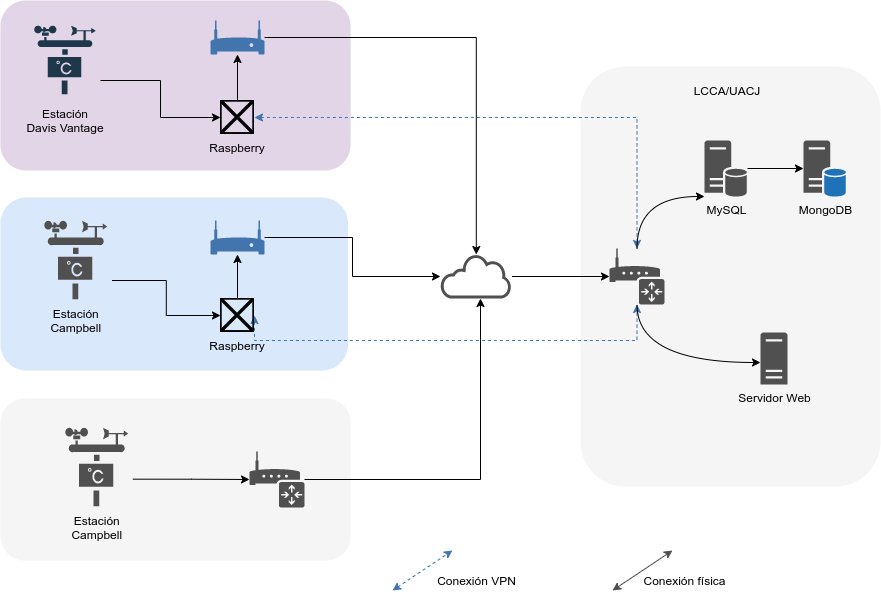
\includegraphics[width=.80\linewidth]{images/diagrams/current_network.png}
	\caption{Diagrama de red de LCCA UACJ.}
	\label{fig:current_network}
\end{figure}

\subsection{Definición del problema}

La falta de una plataforma estandarizada para el monitoreo de las estaciones meteorológicas independiente de las compañías crea un problema de
\cite{muller_sensors_and_the_city}



Debido a la complejidad de los sistemas de monitoreo tecnológico, y al alto grado de conocimiento que es requerido para el monitorear las estaciones y darles mantenimiento. [...] el atender los fallos de las estaciones meteorológicas lleva tiempo y expertise, aún cuando estas fallas no sean críticas o complicadas



Fácil, entendible, UX/UI.

Por lo tanto, se propone la creación de un servicio e interfaz para facilitar la administración y mantenimiento general de los equipos meteorológicos, que *has an objective to aim to a broader audience* para así reducir a los tiempos de respuesta de los fallos de las estaciones meteorológicas.

%! Posibilidad de integrar con FarmOS y otros. Enfocarse en la amplia disponibilidad y accesibilidad general.

%! Tiempo de respuesta como aporte secundario a la metodología
